\documentclass[11pt,a4paper]{article}
\usepackage[T2A]{fontenc}
\usepackage[utf8]{inputenc}
\usepackage[russian]{babel}
\usepackage[margin=2cm]{geometry}
\usepackage{booktabs,graphicx,pdflscape,array,enumitem}
\setlength{\parindent}{0pt}\setlength{\parskip}{4pt}
\setlist{nosep}
\title{Восстановление процесса закупки по журналу событий}
\author{}\date{}
\begin{document}
\maketitle\vspace{-2em}

\section{Данные и метод}
Журнал \texttt{students.csv}: 1000 экземпляров, 6508 событий, 10 активностей, одна версия шаблона. Анализ выполнен на Python (pandas) в Google Colab; ноутбук воспроизводит все числа ниже. Строки группировались по \texttt{ProcessInstanceId} и сортировались по \emph{числовому} \texttt{EventIndex} (индексы достигают двух знаков, лексикографическая сортировка нарушила бы порядок). Из каждого экземпляра получена трасса "--- список \texttt{ActivityName}. Повторы активностей не удалялись: у них разные \texttt{TaskId}, это повторное выполнение. Проверки качества: индексы непрерывны с 1, дублей \texttt{EventId} и пар (экземпляр, индекс) нет, внутри экземпляра время не убывает, одинаковых секунд у соседних событий нет, \texttt{Amount} постоянна внутри экземпляра, все истории начинаются с \texttt{process\_started} и заканчиваются \texttt{process\_completed}. Соответствие \texttt{ActivityName}$\leftrightarrow$\texttt{ActivityId} взаимно однозначно.

\section{Активности, начала и окончания}
Начало одно: \emph{Регистрация заявки} (автоматическое, во всех 1000 экземплярах). Окончаний три, все автоматические: \emph{Заявка выполнена}, \emph{Заявка отклонена}, \emph{Заявка отменена}. Остальные шесть активностей "--- задания людей.

\begin{center}\small
\begin{tabular}{@{}lllp{3.3cm}rr@{}}\toprule
Активность & Код & Роль & Result & Выполнений & Экз.\\\midrule
Регистрация заявки & Рег & \texttt{system} & --- & 1000 & 1000 \\
Первичная проверка & ПП & \texttt{specialist} & accept, reject & 1174 & 1000 \\
Согласование руководителем & СР & \texttt{manager} & accept, cancel, reject, return & 1129 & 955 \\
Проверка бюджета & ПБ & \texttt{finance} & accept & 911 & 911 \\
Дополнительное согласование & ДС & \texttt{director} & accept & 209 & 209 \\
Исполнение закупки & ИЗ & \texttt{procurement} & accept & 911 & 911 \\
Заявка выполнена & ВЫП & \texttt{system} & fulfilled & 911 & 911 \\
Доработка заявки & ДОР & \texttt{requester} & accept & 174 & 156 \\
Заявка отклонена & ОТК & \texttt{system} & rejected & 63 & 63 \\
Заявка отменена & ОТМ & \texttt{system} & cancelled & 26 & 26 \\
\bottomrule\end{tabular}
\end{center}

\section{Основной маршрут и варианты}
Различных полных маршрутов восемь; таблица ниже охватывает все 1000 экземпляров (доли в сумме дают 1; полные названия "--- в \texttt{variants.csv}). Основной маршрут V1 "--- линейная цепочка без возвратов и дополнительного согласования (56,7\%). Остальные варианты "--- это нормальные альтернативы, а не ошибки.

\begin{center}\small
\begin{tabular}{@{}lp{10.8cm}rr@{}}\toprule
Вариант & Маршрут (коды из таблицы выше) & Случаев & Доля\\\midrule
V1 & Рег $\to$ ПП $\to$ СР $\to$ ПБ $\to$ ИЗ $\to$ ВЫП & 567 & 0,567 \\
V2 & Рег $\to$ ПП $\to$ СР $\to$ ПБ $\to$ ДС $\to$ ИЗ $\to$ ВЫП & 188 & 0,188 \\
V3 & Рег $\to$ ПП $\to$ СР $\to$ ДОР $\to$ ПП $\to$ СР $\to$ ПБ $\to$ ИЗ $\to$ ВЫП & 117 & 0,117 \\
V4 & Рег $\to$ ПП $\to$ ОТК & 45 & 0,045 \\
V5 & Рег $\to$ ПП $\to$ СР $\to$ ОТМ & 26 & 0,026 \\
V6 & Рег $\to$ ПП $\to$ СР $\to$ ДОР $\to$ ПП $\to$ СР $\to$ ПБ $\to$ ДС $\to$ ИЗ $\to$ ВЫП & 21 & 0,021 \\
V7 & Рег $\to$ ПП $\to$ СР $\to$ ДОР $\to$ ПП $\to$ СР $\to$ ДОР $\to$ ПП $\to$ СР $\to$ ПБ $\to$ ИЗ $\to$ ВЫП & 18 & 0,018 \\
V8 & Рег $\to$ ПП $\to$ СР $\to$ ОТК & 18 & 0,018 \\
\bottomrule\end{tabular}
\end{center}

Примеры \texttt{ProcessInstanceId} (по одному на вариант):
\begin{itemize}\scriptsize
\item V1: \texttt{00f3e3a0-9d7d-5eac-98a9-b605b6893e61}
\item V2: \texttt{01ae1813-1d99-5524-8f81-77ad5452c33e}
\item V3: \texttt{015bf5dd-d3b4-5b89-8814-7ca369f74e92}
\item V4: \texttt{08a60c66-22dd-5cf8-90dd-71ba3d53f349}
\item V5: \texttt{00e3854b-efb6-59c7-ac6a-c85643843db1}
\item V6: \texttt{055f6c87-61a2-52aa-86ec-940480c96dcd}
\item V7: \texttt{009608ae-1567-584a-b67a-c7ec60ec587d}
\item V8: \texttt{02bf4e3d-60b1-5713-9886-43fa49c67001}
\end{itemize}

\section{Развилки, необязательные этапы, возвраты}
Схема (приложение) содержит три развилки. Это реконструкция по данным: в журнале шлюзов нет.

\textbf{После первичной проверки.} Результат \texttt{accept}: 1129 переходов к согласованию руководителем, \texttt{reject}: 45 переходов к отклонению. Отклонение встречается только на первом проходе, повторная проверка после доработки всегда \texttt{accept}. Сумма заявок при отклонении лежит в диапазоне 8\,272,10--351\,838,75, то есть охватывает практически весь диапазон: по наблюдаемым полям причину выбора ветки назвать нельзя.

\textbf{После согласования руководителем.} Четыре результата: \texttt{accept} (911), \texttt{return} (174, переход к доработке), \texttt{reject} (18) и \texttt{cancel} (26). Отмена и отклонение руководителем встречаются только на первом проходе (в более поздних проходах: 0 случаев). Возврат происходит в 156 из 955 первых проходов и в 18 из 156 вторых; третий проход в журнале всегда заканчивается \texttt{accept}. Суммы при возврате (5\,433,11--384\,811,25), отмене (15\,443,05--387\,374,17) и отклонении (18\,463,41--184\,994,39) перекрываются с суммами принятых заявок, поэтому \texttt{Amount} эти ветки не определяет.

\textbf{После проверки бюджета "--- единственная развилка с подтверждённым правилом.} Дополнительное согласование директором выполняется ровно в тех случаях, когда \texttt{Amount} не меньше порога. Среди 911 заявок, дошедших до проверки бюджета, наибольшая сумма без дополнительного согласования "--- 149\,743,41 ({\scriptsize\texttt{4794f856-d3cb-5466-acf3-94efdfe8b3be}}), наименьшая с ним "--- 150\,614,59 ({\scriptsize\texttt{7c26c98e-2b01-5e87-8b4d-a72a10349271}}); диапазоны не пересекаются. Порог лежит в промежутке между этими числами; круглое значение 150\,000 "--- гипотеза.

\textbf{Обязательные и необязательные этапы.} Всегда: регистрация, первичная проверка и ровно одно из трёх окончаний. Согласование руководителем выполняется не всегда (его нет у заявок, отклонённых на первичной проверке). Проверка бюджета и исполнение закупки есть во всех выполненных заявках и только в них. Дополнительное согласование "--- в 209 заявках, и только для сумм не ниже порога среди дошедших до проверки бюджета (у 19 заявок с большой суммой процесс завершился раньше, до проверки бюджета).

\textbf{Возвраты.} Возврат "--- единственный наблюдаемый цикл: Согласование руководителем $\to$ Доработка заявки $\to$ Первичная проверка $\to$ Согласование руководителем. Он наблюдается в 156 заявках: один раз в 138, два раза подряд в 18; трёх возвратов нет. Доработку выполняет роль \texttt{requester}.

\section{Факт и гипотеза}
\textbf{Наблюдаемый факт:} состав активностей, начала и окончания, все 12 непосредственных переходов, частоты, восемь маршрутов, перечисленные выше правила отсутствия пересечения сумм для ветки дополнительного согласования, отсутствие поздних отмен/отклонений.\\
\textbf{Гипотезы:} (1) точное значение порога суммы (150\,000); (2) причины возврата, отмены и отклонения "--- в журнале нет признака, который их объясняет, возможно, они случайны или определяются ненаблюдаемыми данными; (3) что схема "--- именно исключающие развилки (XOR), а не иной механизм системы; (4) предел в два возврата "--- свойство выборки, процесс мог бы допускать больше. Схема не запрещает отклонение на повторной проверке и третий возврат, хотя в журнале их нет: схема допускает чуть больше, чем наблюдалось.

\section{Ограничения и роль AI}
Выводы о причинах развилок ограничены наблюдаемыми полями (\texttt{Amount}, \texttt{Result}, роль); времена между событиями включают очередь и нерабочее время и для анализа маршрутов не использовались. Схема воспроизводит все 1000 реальных трасс (обратная проверка в ноутбуке), но не доказывает единственность устройства системы.

AI-ассистент (Claude) использовался для разбора условия, составления плана, написания кода ноутбука, подготовки черновика схемы и этого отчёта. Все числа в отчёте пересчитаны по исходному журналу кодом из ноутбука; выводы ассистента о развилках и возвратах проверялись запросами к данным (сводные таблицы по результатам, суммам и номеру прохода), ответы AI в качестве доказательств не использовались.

\begin{landscape}
\section*{Приложение. Схема процесса}
\begin{center}
\IfFileExists{schema.png}{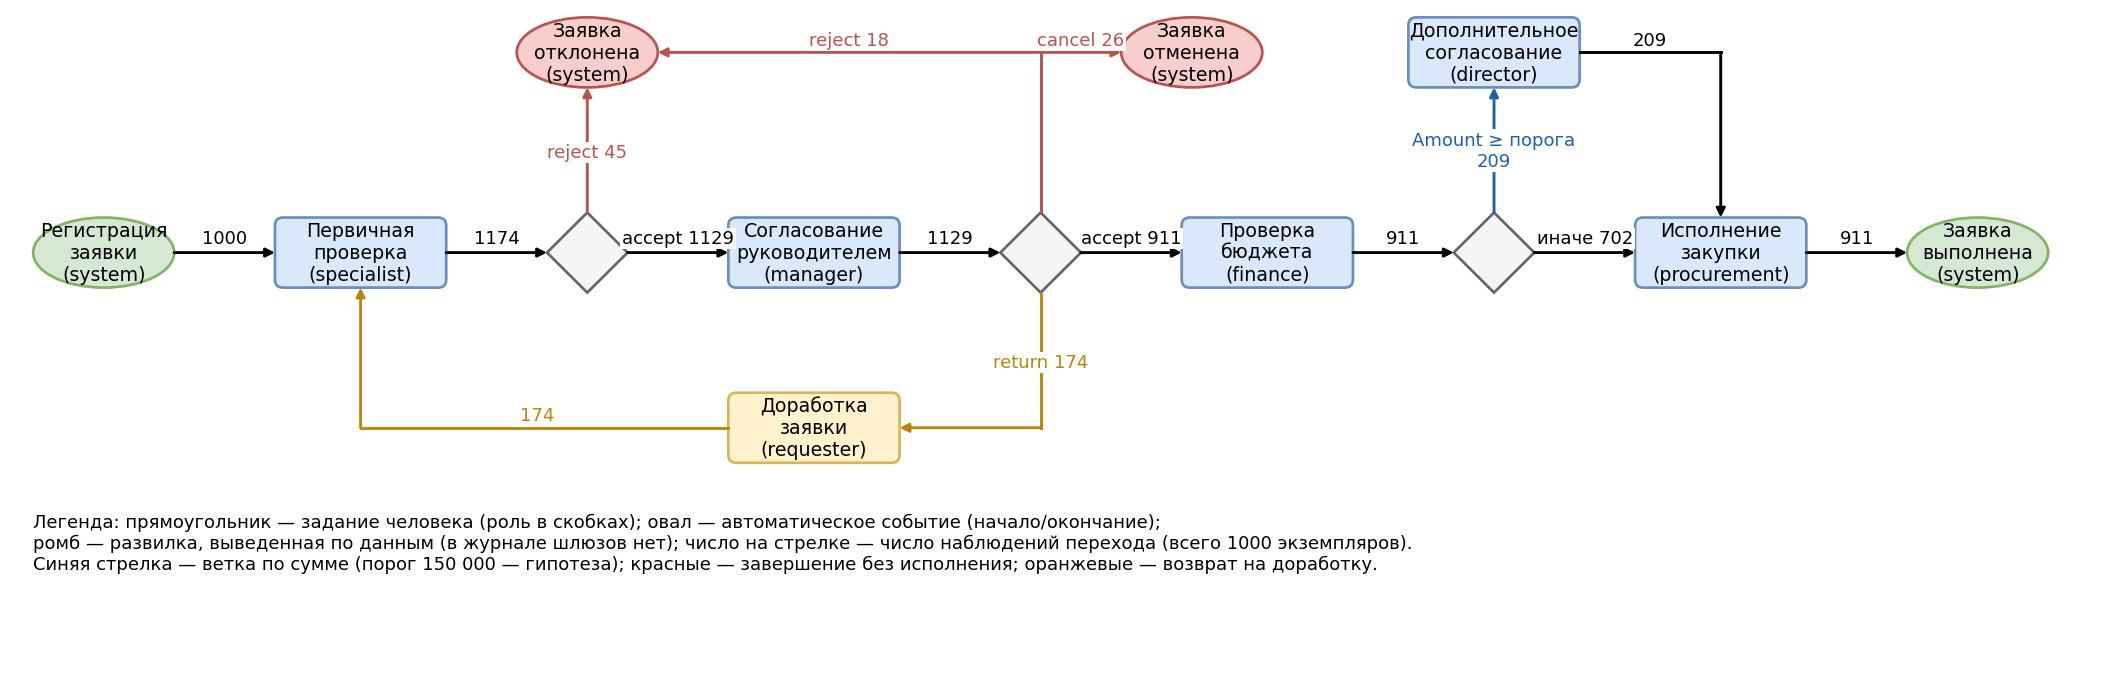
\includegraphics[width=0.97\linewidth]{schema.png}}{\fbox{Положите schema.png рядом с report.tex}}\\[4pt]
\small Редактируемая версия "--- \texttt{schema.drawio}.
\end{center}
\end{landscape}
\end{document}
